\numberwithin{equation}{section}

\section{Revision de la literatura}

El problema de llenado de paquetes en contenedores es también conocido en la literatura como Container Loading Problem o CLP, ha sido ampliamente estudiado desde los años 60's (\textcite{barnett1967exact}), una de las definiciones más sencillas lo realiza \textcite{GEORGE1980147} quién lo define como encontrar posiciones adecuadas para colocar las cajas en el contenedor de tal manera que todas las cajas puedan ser colocadas en el contenedor sin superponerse de tal modo que se maximice la utilización del espacio. A continuación se presentan algunas revisiones de la literatura que se han realizado sobre el problema.

\subsection{Origen del CLP}

El problema de llenado de contenedores tiene su origen en el campo del transporte y la logística. Surge de la necesidad de empacar eficientemente objetos en contenedores o vehículos mientras se optimiza la utilización del espacio. Aunque tiene un origen en la industria, el problema ha sido ampliamente objeto de investigación en la comunidad académica, debido a su complejidad, quienes también los clasifican como un problema de optimización combinatoria derivado de otros problemas de optimización como el problema de cortes y empacado de objetos \textcite{Alvarez-Valdes2018}, el problema de la mochila \textcite{DEQUEIROZ2012200} entre otros.

Existen muchos tipo de problemas de llenado de contenedore, presentaremos a continuación algunas de las clasificaciones más comunes que se han propuesto en la literatura.

\subsection{Formulaciones del CLP}

Muchos de los tipos de problemas formulados en torno al CLP pueden categorizarse en dos tipo principales, los problemas de llenado con restricciones básicas y los problemas de llenado con restricciones prácticas o reales. Los problemas con restricciones básicas son aquellos que consideran restricciones simples, por ejemplo que los paquetes no pueden ser superpuestos y que deben ser colocados dentro de los límites del contenedor, también llamado restricciones de viabilidad del empaquetado \textcite{scheithauer2017introduction}. Los problemas con restricciones prácticas consideran restricciones más realistas como por ejemplo restricciones de estabilidad, restricciones de rotación, restricciones de contigüidad, restricciones de peso, entre otras. 

\textcite{Bortfeldt20131} hizo una revisión de los distintos tipos de restricciones que se han considerado en la literatura, entre las que se encuentran:

\textbf{CLP con múltiples contenedores}: También conocido como el problema de llenado de contenedores múltiples, es una variante del CLP en la que se tienen varios contenedores y se busca llenarlos con un conjunto de paquetes. El objetivo es minimizar el número de contenedores utilizados, maximizando la utilización del espacio en los contenedores.

Algunas de las subvariantes de este problema incluyen el uso de contenedores del mismo tamaño o de diferentes tamaños, por ejemplo Single Bin-Size Bin Packing Problem (SBSBPP) se enfoca en llenar un conjunto de contenedores de un solo tamaño con un conjunto de paquetes (\textcite{ren2011priority}), mientras que Multiple Bin-Size Bin Packing Problem (MBSBPP) se enfoca en llenar un conjunto de contenedores de diferentes tamaños con un conjunto de paquetes (\textcite{zhao2016comparative}).

\textbf{CLP con restricciones de estabilidad}: La estabilidad se refiere a la capacidad de los paquetes de mantenerse en su lugar ya sea en reposo o durante el transporte, evitando movimientos no deseados que puedan dañar la carga o el contenedor. Las restricciones de estabilidad se refieren a las condiciones que deben cumplirse para garantizar que la carga sea estable, como por ejemplo que los paquetes no aplasten, se deslicen o no se caigan.

\textcite{Bortfeldt20131} identifican dos tipos de restricciones de estabilidad: estática y dinámica, señalando que la mayoría de los estudios se concentran en la primera y pocos en la estabilidad dinámica. Critican las métricas de estabilidad existentes por ser insuficientes y no reflejar adecuadamente la estabilidad dinámica real, lo que puede llevar a evaluaciones incorrectas.

\textcite{RAMOS2015480} propone un enfoque para determinar métricas de estabilidad más realistas y aborda la importancia de la estabilidad en las operaciones de carga de contenedores, destacando su impacto en la satisfacción del cliente, la eficiencia operacional y la seguridad de los paquetes y de los operarios. 


\textbf{CLP con restricciones de rotación}: Las restricciones de rotación se refieren a la capacidad de los paquetes de ser rotados en diferentes direcciones, lo que puede aumentar la utilización del espacio y mejorar la estabilidad de la carga. \textcite{Bortfeldt20131} señalan que es un tipo de restricción común en la literatura y que se ha investigado ampliamente, categorizando las restricciones de rotación en 6 tipos:

\begin{itemize}
    \item Caso 1: No se permite rotar las cajas, que deben colocarse en una única orientación fija tanto vertical como horizontalmente.
    \item Caso 2: Solo se permite una orientación vertical fija para cada tipo de caja, pero se pueden rotar 90° en el plano horizontal.
    \item Caso 3: Las cajas pueden rotarse libremente en el plano horizontal y tienen restricciones limitadas en la orientación vertical.
    \item Caso 4: Las cajas pueden tener hasta cinco orientaciones prohibidas en cualquier dirección, permitiendo una amplia variedad de restricciones.
    \item Caso 5: Todas las cajas son completamente rotativas sin restricciones de orientación, proporcionando el máximo grado de libertad.
\end{itemize}

\textbf{CLP con paquetes heterogéneos}: La heterogeneidad de los paquetes se refiere a la variabilidad en las dimensiones, formas y pesos de los paquetes, lo que puede complicar el proceso de empaquetado y afectar la utilización del espacio. \textcite{WASCHER20071109} clasificaron los problemas de llenado de contenedores según la variedad de artículos grandes y pequeños, relacionándolo con el número de diferentes tipos de artículos en el problema y lo clasificaron como: homogéneo (un solo tipo), fuertemente heterogéneo (muchos tipos) o ligeramente heterogéneo (pocos tipos).

\textcite{zhao2016comparative} propusieron una clasificación más detallada basada en la homogeneidad de los contenedores y las cajas, identificando seis subtipos de problemas de llenado de contenedores:

\begin{itemize}
    \item Problema de corte de stock de tamaño único (SSSCSP) si los contenedores son idénticos y las cajas son ligeramente heterogéneas.
    \item Problema de empaque de contenedor de tamaño único (SBSBPP) si los contenedores son idénticos y las cajas son muy heterogéneas.
    \item Problema de corte de stock de múltiples tamaños (MSSCSP) si tanto los contenedores como las cajas son ligeramente heterogéneos.
    \item Problema de empaque de contenedor de múltiples tamaños (MBSBPP) si los contenedores son ligeramente heterogéneos y las cajas muy heterogéneas.
    \item Problema de corte de stock residual (RCSP) si los contenedores son muy heterogéneos y las cajas ligeramente heterogéneas.
    \item Problema de empaque de contenedor residual (RBPP) si tanto los contenedores como las cajas son muy heterogéneos.
\end{itemize}

\subsection{Metodologías de solución}

Muchos autores han propuesto diferentes enfoques heurísticos y metaheurísticos para resolver este problema de manera exacta o aproximada. A continuación se presentan algunas de las metodologías de solución que se han propuesto en la literatura.

\textbf{Métodos exactos}: Los métodos exactos son aquellos que garantizan encontrar la solución óptima al problema, sin embargo, estos métodos pueden ser computacionalmente costosos y no escalables para problemas grandes. Muchos autores han intentado resolver el CLP con restricciones prácticas de manera exacta, pero la mayoría ha encontrado que los métodos exactos no son adecuados para problemas de gran tamaño. Por ejemplo \textcite{JUNQUEIRA201274} mencionan que tuvieron problemas de desbordamiento de memoria al intentar resolver instancias con mas de 20 tipos. Más recientemente \textcite{NASCIMENTO2021105186} propusieron un enfoque exacto basado en modelos de programación lineal entera y programación por restricciones para resolver el problema de llenado de contenedores, demostrando que pudieron resolver instancias de hasta 10 tipos de paquetes y hasta 110 paquetes en un tiempo razonable.

\textbf{Métodos heurísticos}: Los métodos heurísticos son aquellos que no garantizan encontrar la solución óptima, pero pueden proporcionar soluciones de buena calidad en un tiempo razonable. Los métodos heurísticos son ampliamente utilizados para resolver problemas de optimización combinatoria, como el CLP, debido a su eficiencia y escalabilidad. Algunos de los métodos heurísticos constructivos más comunes que se han propuesto en la literatura son: heurística en base a la construcción de paredes \parencite{GEORGE1980147}, con una versión mejorada por \textcite{PISINGER2002382} y heurística en base a la construcción por capas \parencite{BISCHOFF1995377}, con una versión mejorada por \textcite{RANCKJUNIOR2019471}.

\textbf{Métodos metaheurísticos}: El término metaheurística fue acuñado en los años 80s por \textcite{GLOVER1986533}. Una metaheurística puede entenderse como una metodología que incluye estrategias maestras capaces de guiar la búsqueda hacia la solución óptima global. Se consideran más complejas y eficientes que los algoritmos heurísticos simples porque exploran áreas en el espacio de soluciones que van más allá de las exploradas por las heurísticas simples, las cuales tienden a centrarse en encontrar una única solución óptima local. Luego \textcite{Sörensen2013} lo definió como "Un marco algorítmico de alto nivel e independiente del problema que proporciona un conjunto de directrices o estrategias para desarrollar algoritmos de optimización heurísticos". Más recientemente \textcite{MARTI2024} definen una metaheurística no como un algoritmo específico con pasos precisamente definidos, sino como un conjunto más o menos consistente de ideas de alto nivel. Estas ideas sirven como directrices para desarrollar algoritmos de optimización heurísticos ajustados a problemas específicos. En esta definición, se enfatiza la flexibilidad que tiene el diseñador del algoritmo para elegir las características específicas de su método, y se destaca que puede requerirse un grado considerable de "ingeniería" para adaptar el marco de metaheurística a fin de resolver problemas de optimización concretos.

Algunos de los métodos metaheurísticos más comunes que se han propuesto en la literatura para resolver el problema de llenado de contenedores son: 

\begin{itemize}
    \item \textbf{Algoritmos Genéticos (GA)}: Se describe como un algoritmo de búsqueda inspirado en la evolución natural \parencite{goldberg2013genetic}, útil para resolver muchos problemas de optimización debido a su robustez y capacidad de manejar complejidades diversas. Los GA se utilizan en el contexto del CLP para manejar restricciones como el equilibrio de carga, considerado como una restricción estricta en algunos estudios. Por ejemplo algunos autores que han usado GA para resolver el problema de llenado de contenedores son \textcite{RAMOS20181140}, \textcite{GONCALVES2012179}, \textcite{KANG20121287} entre otros.
    \item \textbf{Algoritmos de Enjambre de Partículas (PSO)}: Se describe como un algoritmo de optimización basado en la inteligencia de enjambre, como el de los pájaros o peces. Por ejemplo algunos autores que han usado PSO para resolver el problema de llenado de contenedores son \textcite{KUO2023110417}, \textcite{domingo2012particle}, \textcite{Cano2010} entre otros.
\end{itemize}

\subsection{Software usado en la industria}

En la industria existen varios software que permiten resolver el problema de llenado de contenedores, algunos de los más conocidos son:

\textbf{Cargo Manager}: Según \textcite{zhao2017three}, Cargo Manager (CM) es un ejecutable independiente diseñado para empaquetar contenedores siguiendo un orden de prioridad específico, comenzando por la parte trasera del contenedor. El proceso de empaquetado utiliza una serie de reglas de colocación, probando cada artículo en el orden establecido; si un artículo no es adecuado, se pasa al siguiente, volviendo a considerar los artículos no adecuados en futuras colocaciones. Los artículos de mayor prioridad se empaquetan primero y es posible configurar el sistema para que se adhiera estrictamente a las prioridades de empaque, asegurando que todos los artículos de una prioridad actual se empaquen antes de comenzar con la siguiente.

El proceso principal de empaquetado en CM utiliza diferentes métodos heurísticos constructivos que varían desde heurísticas básicas hasta métodos más complejos y consumidores de tiempo. El objetivo es maximizar el uso del espacio del contenedor formando "muros" con los artículos, donde cada bloque consiste en cajas del mismo tipo y orientación. A medida que se colocan los artículos, los espacios que ocupan ya no están disponibles, generándose nuevos espacios cúbicos que pueden fusionarse con espacios previos. Los métodos difieren en cómo seleccionan los espacios y las cajas, y las restricciones aplicadas al tamaño de los bloques.

En una etapa adicional, CM utiliza la heurística más básica para intentar empaquetar tantos artículos restantes como sea posible. Esta etapa no es adecuada para problemas de múltiples destinos o donde se requiere nivelación de carga, y excluye artículos pesados o frágiles. La solución óptima se determina comparando el volumen y la longitud utilizados por diferentes métodos, seleccionando como mejor aquella solución que ocupe mayor volumen o, en caso de igual volumen, utilice menos longitud. Los usuarios pueden decidir cuántas heurísticas se evalúan, y en caso de seleccionar un solo método, su solución se convierte automáticamente en la solución final. En la imagen \ref{fig:cargomanager} se muestra la interfaz gráfica de Cargo Manager.

\begin{figure}[H]
    \centering
    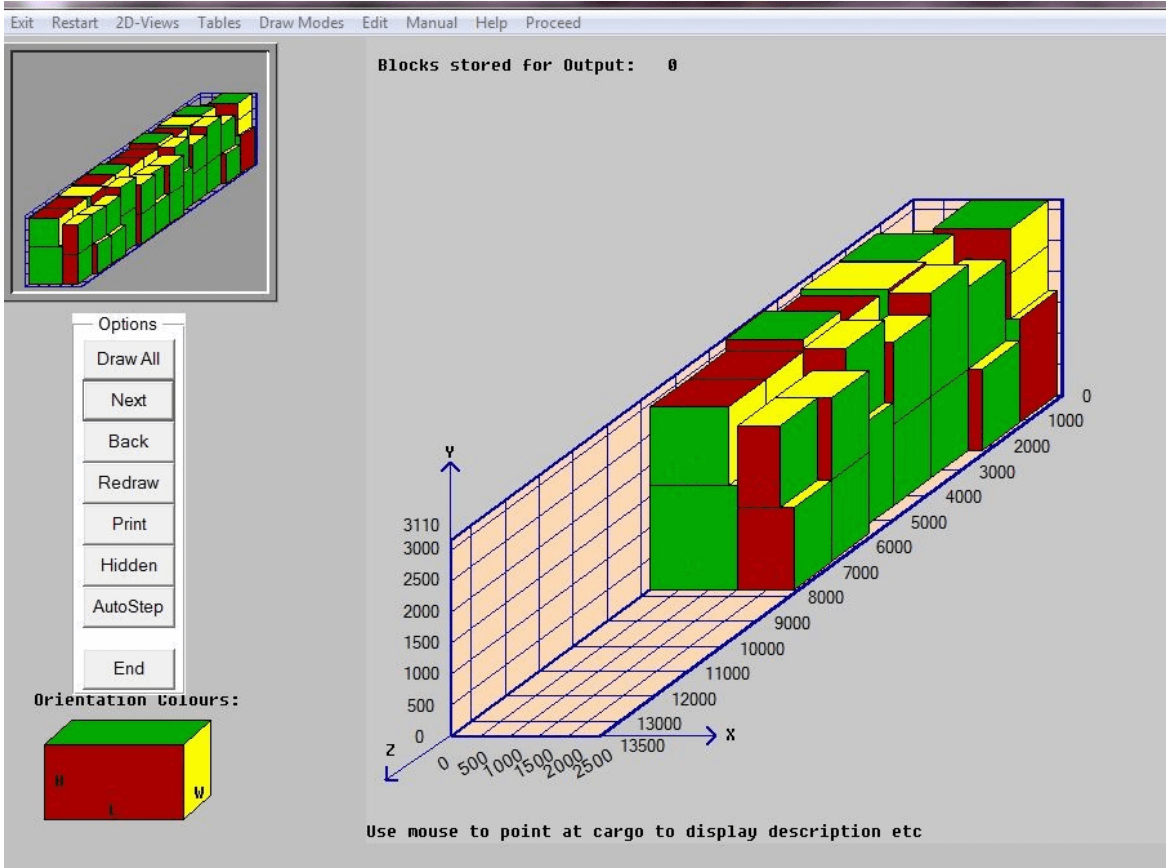
\includegraphics[width=0.8\textwidth]{Figures/cargomanager.png}
    \caption{La interfaz gráfica de Cargo Manager permite a los usuarios empaquetar contenedores siguiendo un orden de prioridad específico, maximizando el uso del espacio y minimizando la longitud utilizada \parencite{zhao2017three}.}
    \label{fig:cargomanager}
\end{figure}

\textbf{PackageCargo}: PackageCargo es una herramienta de apoyo a la decisión, diseñada para abordar el problema de carga de contenedores (CLP), que es esencial en la logística de transporte \parencite{MARTINEZFRANCO2020100601}. Desarrollada como una aplicación de código abierto usando el motor de juegos Unity, esta herramienta permite calcular, visualizar y guardar patrones eficientes de empaque, además de estimar métricas de estabilidad de la carga mediante modelos matemáticos y simulaciones físicas. Su objetivo principal es ofrecer un sistema utilizable tanto en entornos industriales como académicos, permitiendo a los usuarios modificar el marco de trabajo según sus necesidades, lo que ahorra tiempo en desarrollo de software y fomenta la contribución comunitaria para su mejora continua.

El software utiliza un diseño modular que incluye componentes para la visualización de soluciones, simulación de la estabilidad de la carga, y optimización de los patrones de empaque. La arquitectura de PackageCargo facilita la integración de algoritmos de optimización para generar patrones eficientes y su simulación correspondiente para evaluar la estabilidad, usando el motor de físicas PhysX de Nvidia. Esta estructura permite una fácil extensión y adaptación del software, fomentando la innovación y colaboración entre investigadores y profesionales del sector.

PackageCargo no solo ofrece una alternativa competitiva a soluciones comerciales, sino que también se posiciona como una plataforma valiosa para la investigación y el desarrollo en el ámbito del CLP. Al proporcionar una herramienta accesible y extensible, promueve el avance en la comprensión y solución de problemas complejos de carga, beneficiando tanto a la comunidad académica como a la industrial. En la imagen \ref{fig:packagecargo} se muestra la interfaz gráfica de PackageCargo.

\begin{figure}[H]
    \centering
    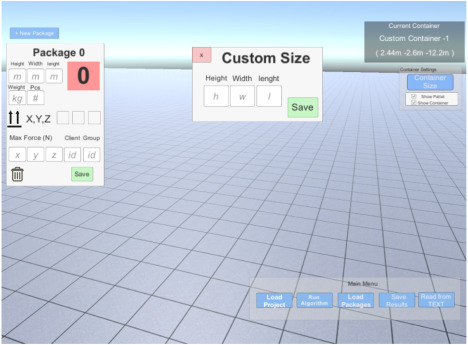
\includegraphics[width=0.8\textwidth]{Figures/packagecargo.jpg}
    \caption{La interfaz gráfica permite al usuario definir variedades de carga, dimensiones, restricciones y cantidades. Esta información se convierte en un archivo de entrada para los algoritmos generadores de patrones de empaque \parencite{MARTINEZFRANCO2020100601}.}
    \label{fig:packagecargo}
\end{figure}


\textbf{LoadCargo}: LoadCargo es un software comercial diseñado para facilitar la planificación y optimización de la carga en contenedores y camiones. Utiliza tecnología en 3D para ofrecer visualizaciones interactivas que mejoran la precisión de las simulaciones de carga. Este sistema admite tanto planificaciones automáticas como manuales, proporcionando herramientas flexibles para diversos requerimientos logísticos \parencite{loadcargo2024}. 

El software es accesible en múltiples plataformas a través de Adobe Air, compatible con sistemas operativos como Windows, Mac OS X y Linux. Soporta tanto unidades métricas como imperiales y se integra con sistemas EDI (Intercambio Electrónico de Datos) para facilitar la importación de datos. Además, incluye características como la visualización del centro de gravedad, exportaciones de planificaciones a varios formatos y herramientas para la construcción de pallets, entre otras. 

LoadCargo es eficaz para optimizar el uso del espacio en contenedores y camiones, aunque mencionan que presenta limitaciones como la incapacidad de manejar cargas de formas irregulares o volúmenes muy altos de cajas. Sin embargo, para operaciones estándar, ofrece soluciones robustas que mejoran la eficiencia en la carga y reducen los costos operativos. En la imagen \ref{fig:loadcargo} se muestra la interfaz gráfica de LoadCargo.

\begin{figure}[H]
    \centering
    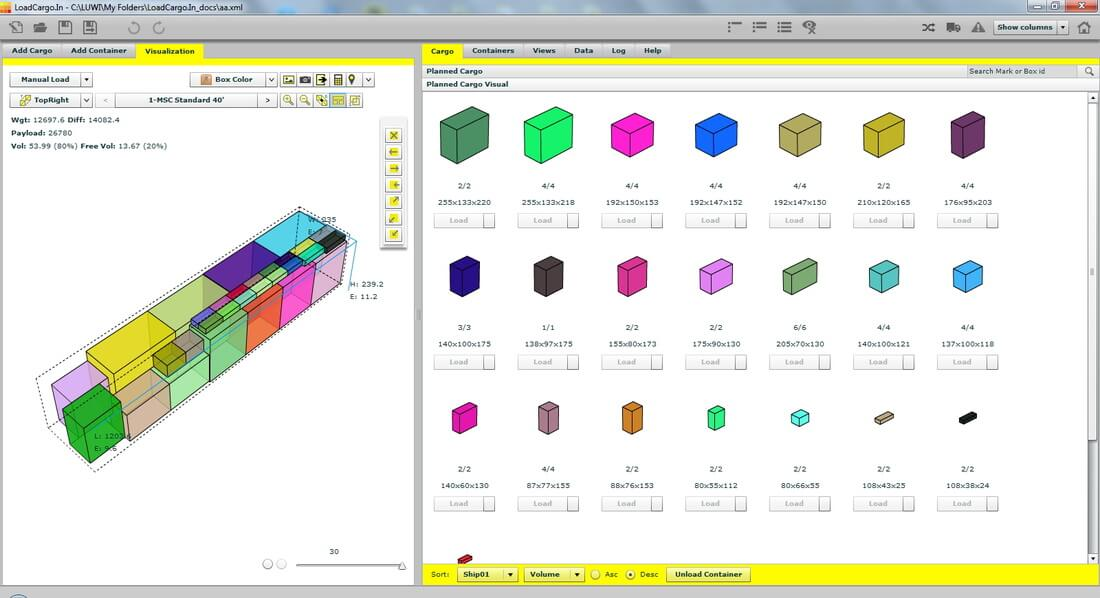
\includegraphics[width=0.8\textwidth]{Figures/loadcargo.jpg}
    \caption{La interfaz gráfica de LoadCargo permite a los usuarios visualizar y planificar la carga de contenedores y camiones, mejorando la eficiencia y reduciendo los costos operativos \parencite{loadcargo2024}.}
    \label{fig:loadcargo}
\end{figure}